\section{Concentric rings}
\label{sec:double_rings}
This section shall discuss the scattering properties of a double-ring structure as depicted in \cref{fig:double_ring_sketch}). 
The geometry consists of a substrate layer sandwiched between two concentric metallic rings of outer radii $R_{1},\,R_{2}$ with widths $w_1,\,w_2$ and a metallic ground plane. The rings, substrate and the metallic ground plane are parallel to the $xy$-plane and stacked in $z$-direction.
The metallic parts i. e. the rings and the ground plane are chosen to possess  the same thickness of $l_z^{\mathrm{R}}$ in $z$-direction, whereas the substrate layer which separates the ground plane and the rings measures $l_z^{\mathrm{S}}$.
The geometry is periodic in both, $x$- and $y$-direction with periodicity $L_\mathrm{x}^\mathrm{UC}$ and $L_\mathrm{y}^\mathrm{UC}$, respectively. Therefore the description of one unit cell is sufficient to discuss the scattering properties of the structure.

Fig. \Ref{fig:artist_view} shows an artist's view of the suggested geometry. Suppose we want to design a metamaterial based on the introduced unit cell which absorbs electromagnetic waves of two different frequencies $f_1$ and $f_2$. How should we choose the size of the unit cell, the layer thicknesses and the ring dimensions? 

It's quite natural that each ring can be capable of supporting circulating currents with a minimum frequency and their corresponding higher harmonics. The radius of the ring sets the resonance frequencies and if we think of the gap between the ground plane and the rings as a resonator the following dependency seems likely:
\begin{equation}
R_i \propto \frac{c}{\pi f_i}.
\label{eqn:radii}
\end{equation}
In \cref{eqn:radii} $c$ denotes the speed of light -- not necessarily its vacuum value. The constant of proportionality can be guessed be physical reasoning. 

An impinging wave of frequency $\omega = 2\pi f$ will induce an electric dipole in each of the rings. If the electrical thickness of the substrate is small compared to the wavelength the metallic backing plane acts as if the induced electric dipole would interact with its mirror image. The situation which occurs is that $z$-directed electric fields build up, which are confinened between each ring and the ground plane.
The length of the resonators is $\pi R_i n^\mathrm{S}$, where $n^\mathrm{S}$ is the (for the moment real) refractive index of the substrate.
From this consideration we end up with the radii:
\begin{equation}
R_i \propto \frac{c}{2 n^\mathrm{S}\pi f_i}.
\label{eqn:radii_precise}
\end{equation}

If we decide to design an absorber operating at the two commonly used wifi frequencies $f_1=2.4$ GHz and $f_2=5.2$ GHz and assume a refractive index of $n^\mathrm{S}$, \cref{eqn:radii_precise} predicts radii of $R_1\approx9.8$ mm and $R_2\approx 4.5$ mm. We could further reduce the parameter space by choosing a square unit cell with $L^\mathrm{UC}_\mathrm{x}=L^\mathrm{UC}_\mathrm{y}=L^\mathrm{UC}\gtrsim 2R_1$. By this choice we maximize the "density" of absorbing rings in the $xy$-plane without shortcutting neighboring rings, what would effectively reduce their length by a factor of $2$.

Since we really do not only conduct a theoretical analysis but rather want to manufacture the absorber by a PCB layout, we are quite limited in the choice of the substrate and the available board thicknesses. Lets choose $l_z^\mathrm{S}=2$ mm and take FR4 with real part of permittivity $\epsilon_\mathrm{r}=4.4$ and a loss tangent of $\tan \delta=0.02$. The metallic character of copper shall be incorported by setting its conductivity $\sigma=55\times 10^6$ S/m. This corresponds to a purely imaginary permittivity $\epsilon/\epsilon_0 = \imag \sigma$ relative to the permittivity of vacuum $\epsilon_0$.

\begin{figure}
\centering
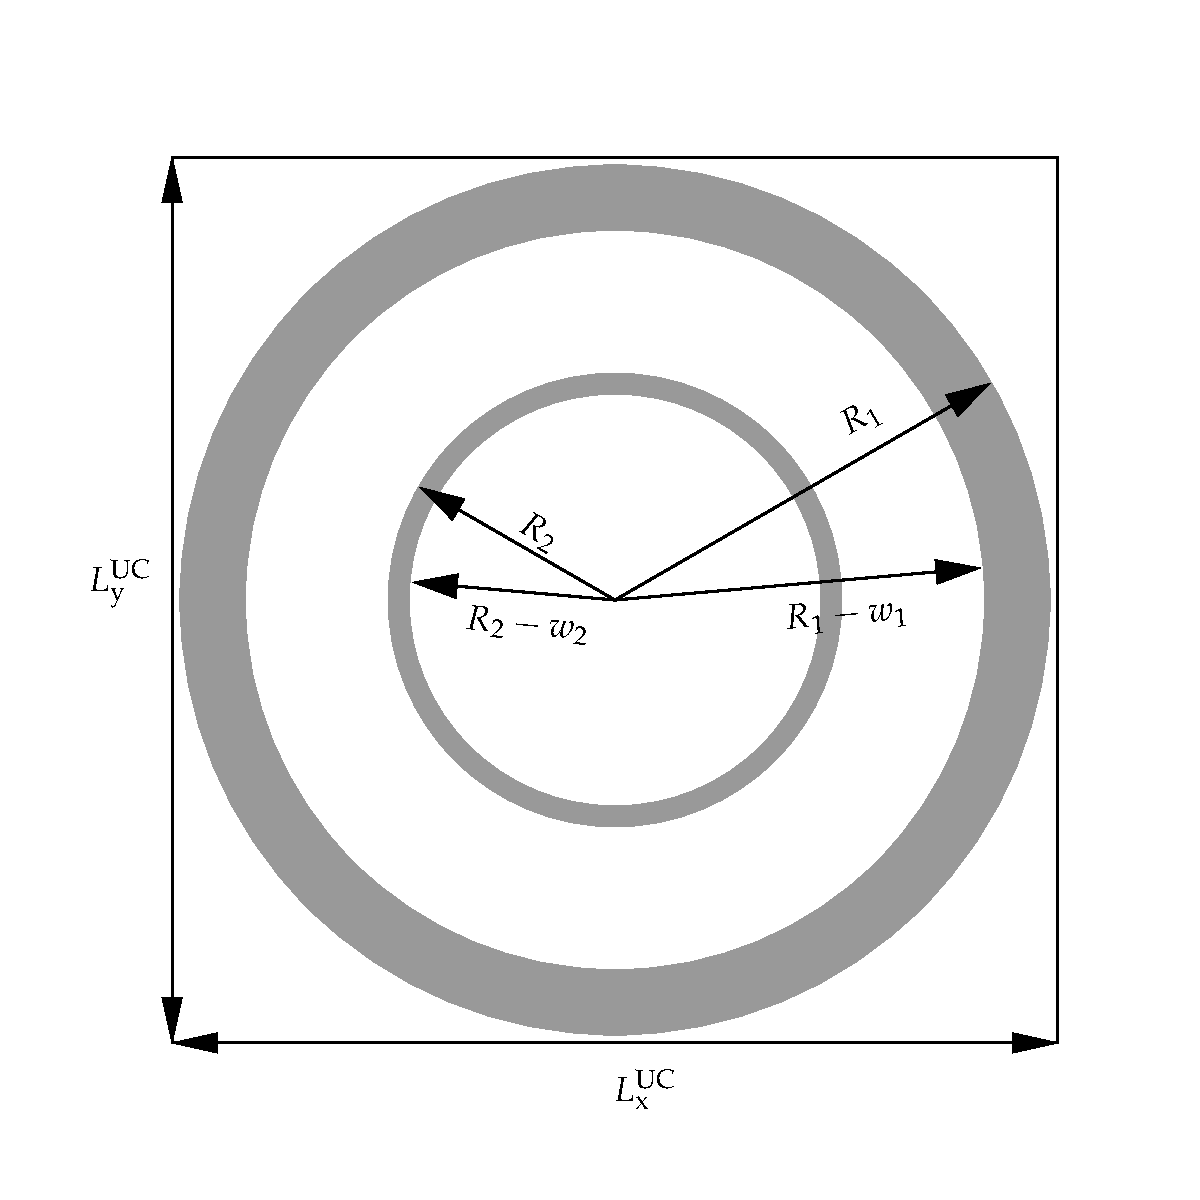
\includegraphics[width=0.75\linewidth]{./media/double_ring_sketch.pdf}
\caption{Two concentric rings of outer radii $R_1$, $R_2$ with widths $w_1$, $w_2$ constitute a metamaterial unit cell with edge lengths of $L_\mathrm{x}^\mathrm{UC}$, $L_\mathrm{y}^\mathrm{UC}$ in $x$- and $y$-direction.}
\label{fig:double_ring_sketch}
\end{figure}

\begin{figure}
\centering
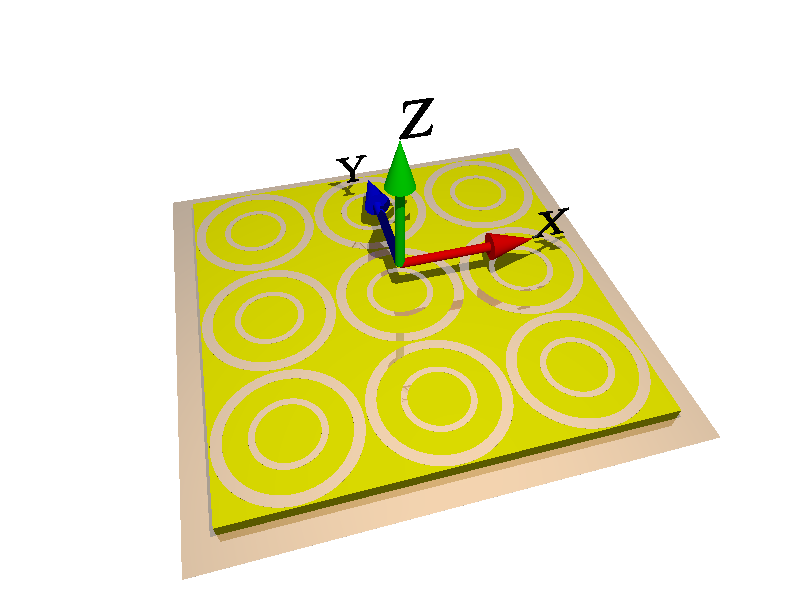
\includegraphics[width=0.75\linewidth]{./media/double_rings.png}
\caption{An artist's view of the suggested metamaterial absorber consisting of a FR4 substrate (yellow) sandwiched between concentric copper rings and a copper backing plane.}
\label{fig:artist_view}
\end{figure}

\subsection{Parameter studies}
In order to find out how the various parameters influence the absorption properties this chapter shows some numerical results for the reflection parameter $S_{11}$.
\capFref{fig:w1_sweep} shows the absolute value of $S_{11}$ as a function of frequency for a fixed outer ring radius of $R_1=9.8$ mm but changing width $w_1$. As we can see there are several additional drops in the scattering parameter including the desired peaks at about 2.4 and 5.2 GHz. Since the 5.2 GHz peak is contributed by the smaller ring changing the width of the larger ring does hardly influence the scattering behaviour at this frequency, whereas at all other frequencies $f<15$ GHz a shift to higher values of $f$ is observed upon an increase of $w_1$.

\begin{figure}
\centering
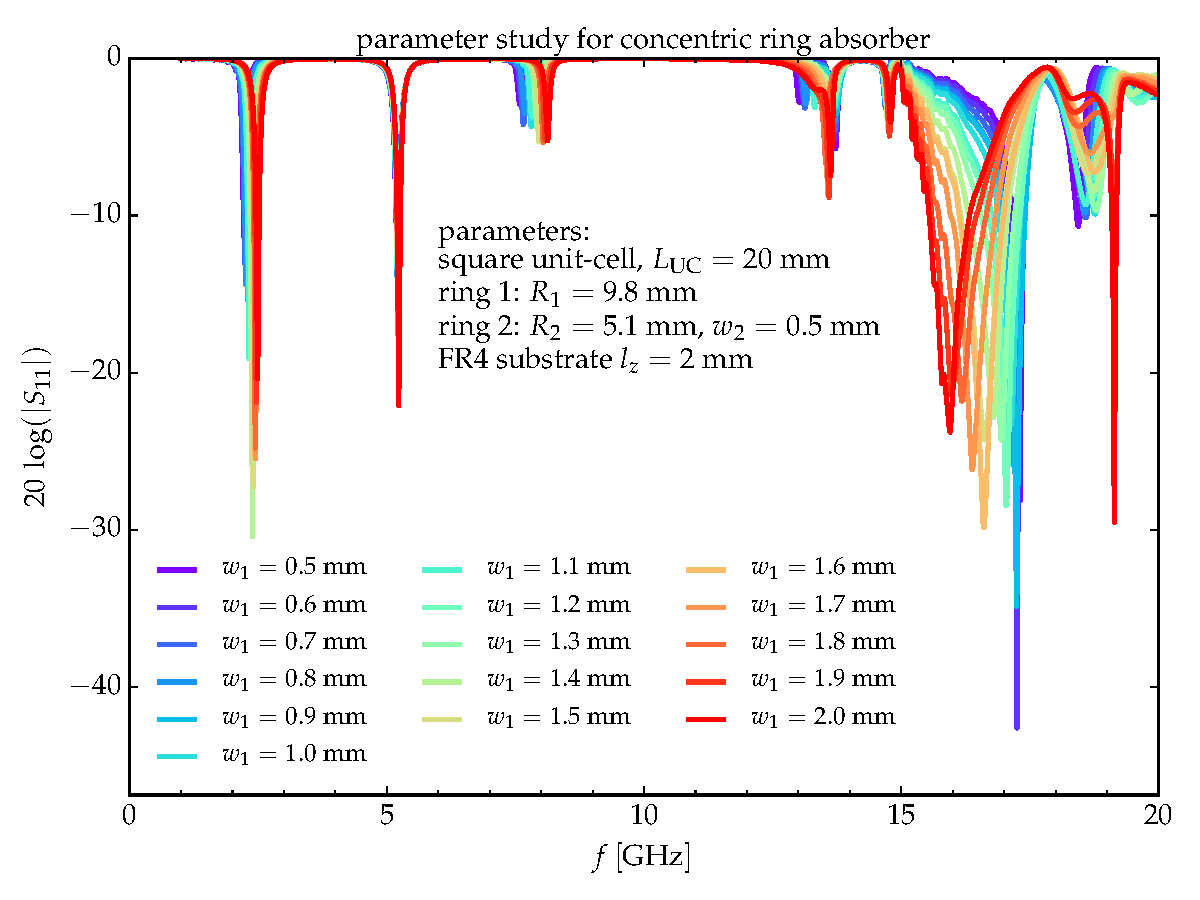
\includegraphics[width=0.75\linewidth]{./media/dual-wifi_absorber_w1.pdf}
\caption{Influence of the larger ring width upon the scattering properties of the concentric ring metamaterial.}
\label{fig:w1_sweep}
\end{figure}

\begin{figure}
\centering
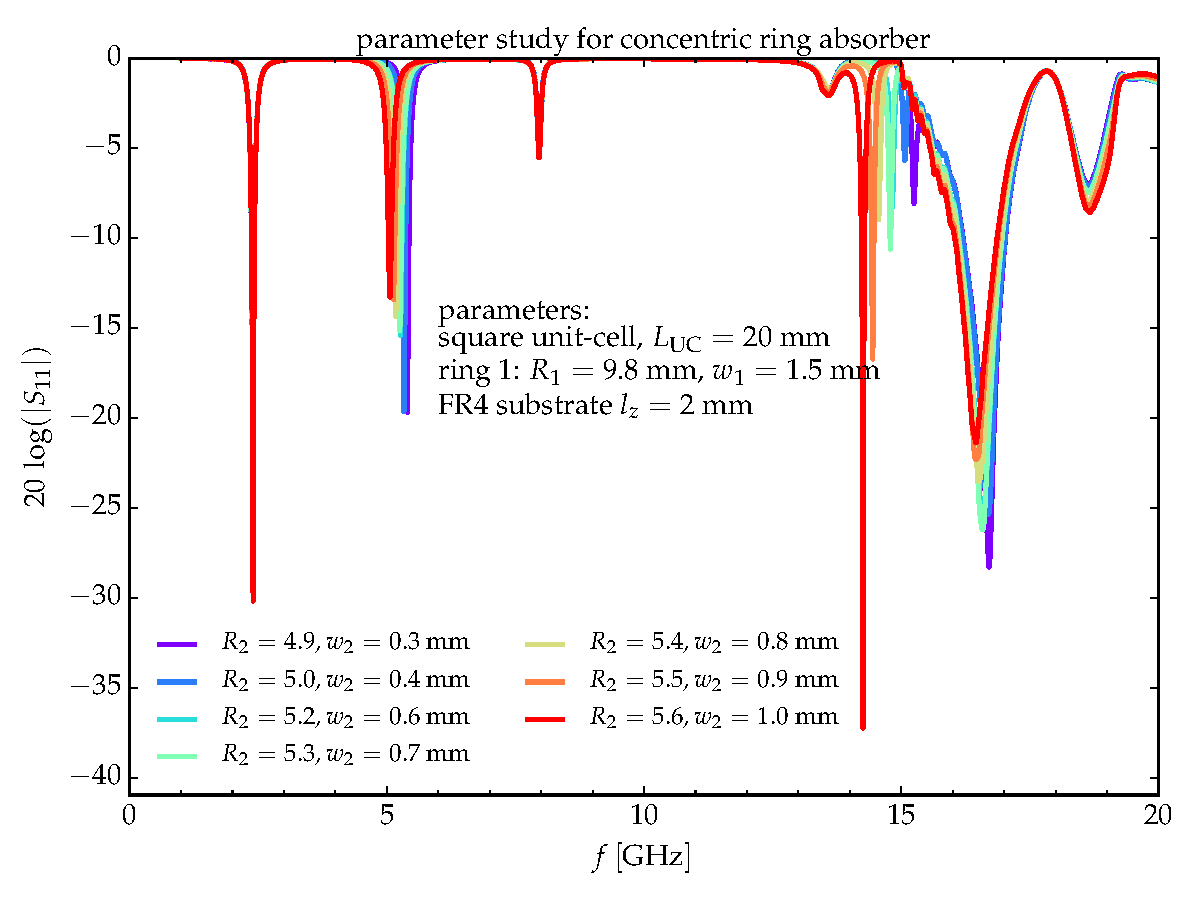
\includegraphics[width=0.75\linewidth]{./media/dual-wifi_absorber_w2.pdf}
\caption{Influence of the smaller ring width upon the scattering properties of the concentric ring metamaterial. In contrast to the study of \Cref{fig:w1_sweep} not the outer, but the inner radius is kept at the value $R_{2i}=4.6$ mm.}
\label{fig:w2_sweep}
\end{figure}

As we would expect a variation of the width of the smaller ring follows the analogous reasoning. \capFref{fig:w2_sweep} exemplifies this behaviour and depicts the absolute value of $S_{11}$ as a function of frequency for a fixed smaller ring radius of $R_{2i}=4.6$ mm but changing width $w_2$. Since this time a second peak, namely the one at approximately 8 GHz doesn't show a dependence upon $w_2$ we can conclude it is associated to a higher harmonic of the larger ring. 

To discriminate the influence of both rings \Cref{fig:single_double_rings} shows the absolute value of the scattering parameter of two isolated rings (solid color lines) and the concentric ring configuration (dashed black line) as functions of frequency.

\begin{figure}
\centering
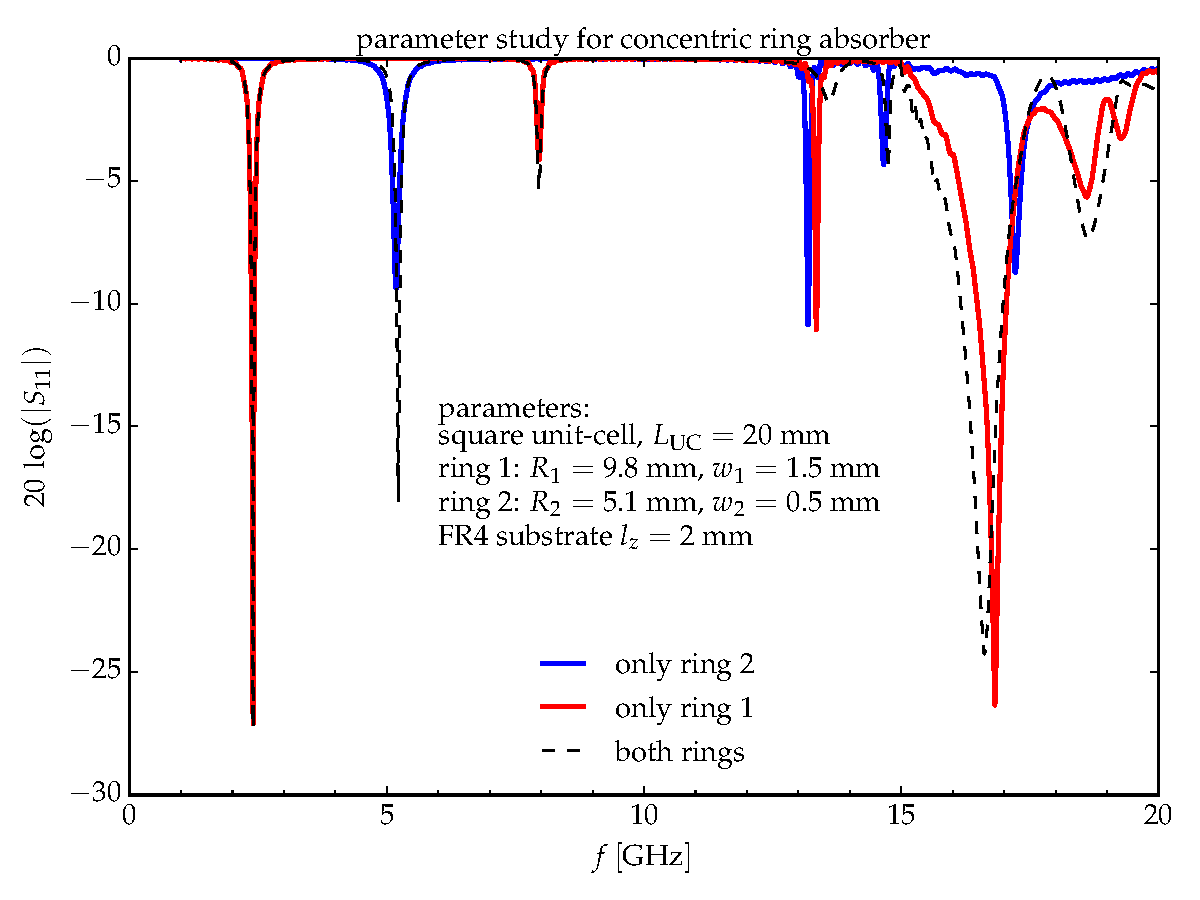
\includegraphics[width=0.75\linewidth]{./media/wifi_absorber_single_double_rings.pdf}
\caption{Comparision of $|S_{11}|$ for an isolated ring 1 with $R_1=9.8$ mm, $w_1=1.5$ mm (red solid), ring 2, $R_2=5.1$ mm, $w_2=0.5$ mm (blue solid) and the concentric configuration (black dashed), where both rings are present.}
\label{fig:single_double_rings}
\end{figure}

To study how the size of the unit-cell influences the position of the absorption 
minima of the double--ring--absorber, \Cref{fig:LUC} shows the position of the two first absorption maxima at about $f_1\approx2.7$ GHz and $f_2\approx 5.5$ GHz as a function of the size of the unit cell, $L^\text{UC}$.
\begin{figure}
\centering
\includegraphics[width=0.75\linewidth]{./media/Einfluss_LUC.pdf}
\caption{Simulated position of the first two absorption maxima of a double ring absorber with $R_1=9.8$ mm, $w_1=1.5$ mm, $R_2=5.1$ mm, $w_2=0.5$ mm as a function of the size of the a-dimension. Metallic parts are chosen to be copper and FR4 is supposed to possess $\Re\left(\epsilon\right)=4.1$ and a loss tangent $\tan\delta = 0.015$.}
\label{fig:LUC}
\end{figure}

What can be observed is that as the size of the unit cell grows, the absorption frequency which can be attributed to the larger ring suffers a shift to higher frequencies. Since this shift tends to saturate as the distance of the outer ring to its neighbours becomes comparable to the ring radius. Therefor we can say that a stronger coupling of neighbouring unit cells leads to an increase of the resonance frequency of the larger ring, whereas the resonance frequency of the smaller ring does not show a significant dependence on the size of the unit cell. This is probably the case since $L^\mathrm{UC}/2 R_2\gtrsim 1.8$ even for the smallest unit cell with $L^\mathrm{UC}=20$ mm, where the beginning of the saturation in \Cref{fig:LUC} is way back.

What is of interest, too is the magnitude of the absorption at the two resonant frequencies as the unit cell grows. \capFref{fig:LUC_absS11} shows this dependence.

\begin{figure}
\centering
\includegraphics[width=0.75\linewidth]{./media/Einfluss_LUC_absS11.pdf}
\caption{Simulated ratio of $|S_{11}(\eta)|/|S_{11}(\eta=1.02)|$ for the first two absorption maxima of a double ring absorber with $R_1=9.8$ mm, $w_1=1.5$ mm, $R_2=5.1$ mm, $w_2=0.5$ mm as a function of the size of the a-dimensional parameter $\eta = L^\mathrm{UC}/2R_1$. Metallic parts are chosen to be made of copper and FR4 is supposed to possess $\Re\left(\epsilon_\mathrm{r}\right)=4.1$ and a loss tangent $\tan\delta = 0.015$.}
\label{fig:LUC_absS11}
\end{figure}


\subsection{Comparison to measured data}
Due to the promising absorption characteristics of the discussed absorber it has been manufactured and measured experimentally. The magnitude of the measured and simulated values of $S_{11}$ are depicted in 